


\documentclass[]{article}
\usepackage{pgfplots}
\begin{document}
\section{inset figure2}
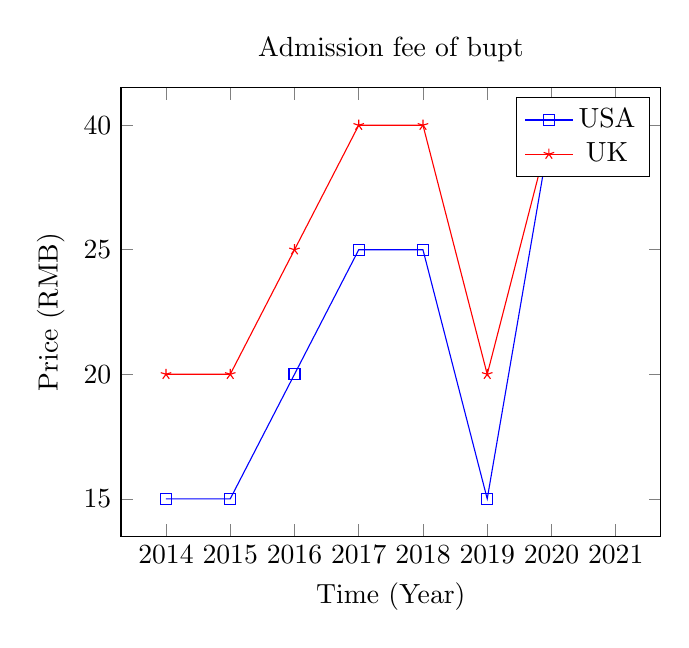
\begin{tikzpicture}
\begin{axis}
[title={Admission fee of bupt},
xlabel={Time (Year)},
ylabel={Price (RMB)},
xtick={1,	2,	3,	4,	5,	6, 7, 8},
ytick={1,	2,	3,	4},
xticklabels={2014, 2015, 2016, 2017, 2018, 2019, 2020, 2021},
yticklabels={15, 20, 25, 40}
]
\addplot[color=blue,mark=square]
coordinates {
	(1,1)	(2,1)	(3,2)	(4,3)	(5,3)	(6,1) (7,4)	(8,4)
};
\addplot[color=red,mark=star]
coordinates {
	(1,2)	(2,2)	(3,3)	(4,4)	(5,4)	(6,2) (7,4)	(8,4)
};
\legend{USA, UK}
\end{axis}
\end{tikzpicture}
\end{document}




%\addplot[color=blue,mark=square,]
%coordinates {
%	(1,1)	(2,1)	(3,2)	(4,3)	(5,3)	(6,1) (7,4)	(8,4)
%};
%xtick={1,	2,	3,	4,	5,	6},
%ytick={15,	20,	25,	40},
